% 第6章第1节：特征值与特征向量（特征方向、特征空间、特征多项式与Cayley--Hamilton定理、相似不变性、不同特征值的特征向量）。

\section{特征值与特征向量}
\label{sec:ls-linear-operators}

第~\ref{sec:ls-similarity}节的例子已经显示，算子$T(x_1,x_2)=(2x_1+x_2,3x_2)$在标准基下的矩阵有非零的非对角元，换到新基$\bm b_1'=\bm e_1$、$\bm b_2'=\bm e_1+\bm e_2$以后却成了对角矩阵$\operatorname{diag}(2,3)$。原因在于，这两个基方向在作用下只被伸缩、不被转向。不过，那组新基是事先给出、再加以验证的。要为一般的算子找出这样的基，需要依次回答四个问题：只被伸缩的方向怎样寻找，伸缩倍数怎样求出，它们是否随基改变，彼此线性无关的这类方向最多有多少个。

\subsection{只被伸缩的方向}
\label{sec:ls-operator-eigenvectors}

第~\ref{sec:ls-linear-map-definition}节说明，线性算子$T:V\to V$总把原点留在原处，但一般会同时改变向量的长度和方向。于是可以问：有没有非零向量在作用以后仍落在原来那条过原点的直线上，只被伸长、缩短或反向，而不被转到别的方向？用等式表达，就是要求非零向量$\bm v\in V$与实数$\lambda$满足
\begin{equation}
 T\bm v=\lambda\bm v,\qquad \bm v\neq\bm0.
 \label{eq:matrix-analysis-eigenpair}
\end{equation}
这时称$\lambda$为$T$的\term{特征值}（eigenvalue），$\bm v$为属于$\lambda$的\term{特征向量}（eigenvector），$\bm v$所在的直线称为\term{特征方向}。

特征值说明这条直线上发生了什么：$|\lambda|>1$时向量被拉长，$|\lambda|<1$时被缩短，$\lambda<0$时方向还被反过来，$\lambda=0$则表示$T\bm v=\bm0$，即$\bm v$在$T$的核中。定义要求特征向量非零，因为零向量对任何$\lambda$都满足$T\bm0=\lambda\bm0$，不提供方向信息。

在特征方向上，反复作用也最简单。第~\ref{sec:ls-operator-powers}节说明，算子可以与自身复合，得到$T^k$。对特征向量$\bm v$，由$T\bm v=\lambda\bm v$与线性性得$T^2\bm v=T(\lambda\bm v)=\lambda T\bm v=\lambda^2\bm v$，归纳即得$T^k\bm v=\lambda^k\bm v$。所以在这条直线上，$k$次作用化为数$\lambda$的$k$次乘方；在一般方向上，矩阵幂则会不断混合各个坐标。

特征值是算子本身的性质，不依赖基的选取。取一组基$\mathcal B$后，式~\eqref{eq:matrix-analysis-eigenpair}的坐标形式是$[T]_{\mathcal B}[\bm v]_{\mathcal B}=\lambda[\bm v]_{\mathcal B}$。等式两侧分别是向量$T\bm v$与$\lambda\bm v$的坐标，而$\bm v\neq\bm0$当且仅当它的坐标非零。所以无论取哪组基，矩阵$[T]_{\mathcal B}$的特征值都恰好是$T$的特征值；换基只改变特征向量的坐标。对$n$阶方阵$\bm A$，它的特征值与特征向量指算子$\bm x\mapsto\bm A\bm x$的特征值与特征向量，即满足$\bm A\bm v=\lambda\bm v$、$\bm v\neq\bm0$的$\lambda$与$\bm v$。

回到开头的算子，可以直接验证哪些方向是特征方向。
\begin{example}[验证特征向量]
\label{ex:ls-operator-eigenvector-check}
给定算子$T(x_1,x_2)=(2x_1+x_2,3x_2)$，它在标准基下的矩阵为
\[
 \bm A=\begin{bmatrix}2&1\\0&3\end{bmatrix}.
\]
检验$\bm e_1$、$(1,1)^{\top}$与$\bm e_2$是否为特征向量。直接相乘得
\[
 \bm A\bm e_1=\begin{bmatrix}2\\0\end{bmatrix}=2\bm e_1,\qquad
 \bm A\begin{bmatrix}1\\1\end{bmatrix}=\begin{bmatrix}3\\3\end{bmatrix}=3\begin{bmatrix}1\\1\end{bmatrix},\qquad
 \bm A\bm e_2=\begin{bmatrix}1\\3\end{bmatrix}.
\]
结论：$\bm e_1$与$(1,1)^{\top}$是特征向量，特征值分别为$2$和$3$，它们正是第~\ref{sec:ls-similarity}节新基的两个方向；$(1,3)^{\top}$不是$\bm e_2$的倍数，所以$\bm e_2$不是特征向量。
\end{example}
图~\ref{fig:ls-operator-eigenvectors}画出这个例子：两条特征方向上的向量作用后仍在原直线上，只是变长；其他方向上的向量则被转开。
\begin{figure}[!htb]
  \centering
  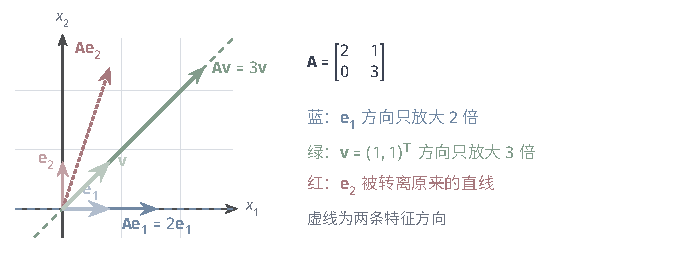
\includegraphics[width=112mm]{figures/01-mathematical-preliminaries-upper/03-linear-spaces/tikz/comprehension-additions/operator-eigenvectors.pdf}
  \caption{特征向量只被伸缩、不被转向。算子$T(x_1,x_2)=(2x_1+x_2,3x_2)$在标准基下的矩阵为$\bm A=\left[\begin{smallmatrix}2&1\\0&3\end{smallmatrix}\right]$，它把$\bm e_1$送到$2\bm e_1$，把$\bm v=(1,1)^{\top}$送到$3\bm v$，二者都留在各自的虚线上；$\bm e_2$被送到$(1,3)^{\top}$，偏离了原来的直线，所以不是特征向量。}
  \label{fig:ls-operator-eigenvectors}
\end{figure}

并非每个算子都有实特征向量。下面的反例中，每个非零向量都被转离原来的直线。
\begin{example}[反例：平面旋转没有实特征向量]
\label{ex:ls-rotation-no-real-eigenvector}
给定平面上逆时针旋转$90^\circ$的算子$R(x_1,x_2)=(-x_2,x_1)$。检验它是否有实特征值。设实数$\lambda$与向量$(x_1,x_2)$满足$R(x_1,x_2)=\lambda(x_1,x_2)$，即
\[
 -x_2=\lambda x_1,\qquad x_1=\lambda x_2 .
\]
把第二式代入第一式得$-x_2=\lambda^2x_2$，即$(1+\lambda^2)x_2=0$。由于$1+\lambda^2>0$，只能$x_2=0$，进而$x_1=\lambda x_2=0$。结论：对任何实数$\lambda$，满足等式的只有零向量，所以$R$没有实特征值，也没有实特征向量。
\end{example}

\subsection{特征空间与不变子空间}

同一个特征值往往不止对应一条特征方向。固定特征值$\lambda$，满足$T\bm v=\lambda\bm v$的全部向量连同零向量组成集合$\ker(T-\lambda\,\operatorname{id}_V)$，称为$\lambda$的\term{特征空间}（eigenspace）。它是一个线性映射的核，因而是子空间。例如$\bm I_2$的每个非零向量都是属于$1$的特征向量，特征空间是整个平面；而示例~\ref{ex:ls-operator-eigenvector-check}中属于$2$的特征空间只是$\bm e_1$所在的直线，因为$\bm A-2\bm I=\left[\begin{smallmatrix}0&1\\0&1\end{smallmatrix}\right]$的核由第二坐标为零的向量组成。

特征空间是一类更一般的子空间的特例。若子空间$S$满足$T(S)\subseteq S$，就称$S$为$T$的\term{不变子空间}（invariant subspace）。这时作用不会把$S$中的向量带出$S$，于是可以把$T$限制在$S$上单独研究。特征空间是不变子空间，因为其中的向量只被乘以$\lambda$，仍留在其中。

一维不变子空间恰好就是特征方向。若$\bm v\neq\bm0$且$\operatorname{span}\{\bm v\}$不变，则$T\bm v$落在这条直线上，是$\bm v$的倍数；反之，若$T\bm v=\lambda\bm v$，则$T(c\bm v)=\lambda c\bm v$仍在这条直线上。高于一维的不变子空间却未必含有特征方向：整个平面对$90^\circ$旋转不变，而示例~\ref{ex:ls-rotation-no-real-eigenvector}说明其中没有一条特征方向。第~\ref{sec:ls-general-square-spectrum}节将看到，这样的二维不变子空间对应一对共轭的复特征值。

\subsection{特征多项式}
\label{sec:ls-characteristic-polynomial}

示例~\ref{ex:ls-operator-eigenvector-check}中的特征向量是先猜出、再验证的。能否系统地求出全部特征值？对$n$阶方阵$\bm A$，$\lambda$是特征值，当且仅当齐次方程$(\bm A-\lambda\bm I)\bm v=\bm0$有非零解，即$\ker(\bm A-\lambda\bm I)\neq\{\bm0\}$。由第~\ref{sec:ls-injective-surjective-invertible}节的等价条件，这又等价于$\operatorname{rank}(\bm A-\lambda\bm I)<n$，也等价于$\bm A-\lambda\bm I$不可逆。

不可逆又等价于行列式为零，这一步用到第~\ref{sec:ls-determinant-properties}节的两条性质。若方阵$\bm M$可逆，乘法性给出$\det\bm M\det(\bm M^{-1})=\det\bm I=1$，故$\det\bm M\neq0$；反之若$\det\bm M\neq0$，古典伴随恒等式说明$\operatorname{adj}(\bm M)/\det\bm M$就是$\bm M$的逆。所以$\lambda$是$\bm A$的特征值，当且仅当$\det(\bm A-\lambda\bm I)=0$。第~\ref{sec:ls-similarity-properties}节把每个$\operatorname{rank}(\bm A-c\bm I)$都列为相似不变量；现在可以看出，使这个秩小于$n$的数$c$恰好就是特征值。

为了把这个条件写成首项系数为正的多项式，注意$\det(\lambda\bm I-\bm A)=(-1)^n\det(\bm A-\lambda\bm I)$，二者同时为零。定义
\begin{equation}
 p_{\bm A}(z)=\det(z\bm I-\bm A),
 \label{eq:matrix-analysis-characteristic-polynomial}
\end{equation}
称为\term{特征多项式}（characteristic polynomial），就得到：$\bm A$的实特征值恰为$p_{\bm A}$的实根。在行列式的排列展开中，对角线一项是$\prod_i(z-a_{i,i})$；其余每一项至少有两个因子取自非对角位置，含$z$的因子至多$n-2$个。所以只有对角线一项含$z^n$，$p_{\bm A}$是首项系数为$1$的$n$次实多项式，至多有$n$个不同的根。求出一个特征值$\lambda$以后，再解齐次方程$(\bm A-\lambda\bm I)\bm v=\bm0$，就得到它的特征空间。

用特征多项式可以重新求出前面两个例子的特征值，而不必猜测特征向量。
\begin{example}[用特征多项式求特征值]
\label{ex:ls-characteristic-polynomial-two-by-two}
给定示例~\ref{ex:ls-operator-eigenvector-check}的$\bm A=\left[\begin{smallmatrix}2&1\\0&3\end{smallmatrix}\right]$，以及示例~\ref{ex:ls-rotation-no-real-eigenvector}的旋转在标准基下的矩阵$\bm R=\left[\begin{smallmatrix}0&-1\\1&0\end{smallmatrix}\right]$。二者的特征多项式为
\[
 \begin{aligned}
 p_{\bm A}(z)&=\det\begin{bmatrix}z-2&-1\\0&z-3\end{bmatrix}=(z-2)(z-3),\\
 p_{\bm R}(z)&=\det\begin{bmatrix}z&1\\-1&z\end{bmatrix}=z^2+1 .
 \end{aligned}
\]
结论：$\bm A$的特征值为$2$与$3$，与示例~\ref{ex:ls-operator-eigenvector-check}验证的两条特征方向相符；$z^2+1$对任何实数$z$都为正，没有实根，所以$\bm R$没有实特征值，与示例~\ref{ex:ls-rotation-no-real-eigenvector}的直接验证一致。
\end{example}
$\bm A$的情形可以推广到任意三角矩阵：三角矩阵$\bm A$的$z\bm I-\bm A$仍是三角矩阵，行列式是对角元之积$\prod_i(z-a_{i,i})$，所以三角矩阵的特征值就是它的对角元。

特征多项式在每个特征值处取零。若把矩阵本身代入特征多项式，又会得到什么？这里的代入是指把多项式中的$z^j$换成$\bm A^j$，常数项$c_0$换成$c_0\bm I$。先看一个例子。
\begin{example}[把矩阵代入它的特征多项式]
\label{ex:ls-cayley-hamilton-two-by-two}
给定$\bm A=\left[\begin{smallmatrix}2&1\\0&3\end{smallmatrix}\right]$。由示例~\ref{ex:ls-characteristic-polynomial-two-by-two}，$p_{\bm A}(z)=(z-2)(z-3)=z^2-5z+6$。计算$p_{\bm A}(\bm A)=\bm A^2-5\bm A+6\bm I$：
\[
 \bm A^2=\begin{bmatrix}4&5\\0&9\end{bmatrix},\qquad
 \bm A^2-5\bm A+6\bm I
 =\begin{bmatrix}4-10+6&5-5+0\\0&9-15+6\end{bmatrix}
 =\bm0 .
\]
结论：把$\bm A$代入自身的特征多项式，得到零矩阵。
\end{example}
这不是巧合。证明的工具是第~\ref{sec:ls-determinant-properties}节的古典伴随恒等式（定理~\ref{thm:ls-adjugate-identity}）$\bm M\operatorname{adj}(\bm M)=\det(\bm M)\bm I$。令$\bm M=z\bm I-\bm A$，得
\[
 (z\bm I-\bm A)\operatorname{adj}(z\bm I-\bm A)=p_{\bm A}(z)\bm I .
\]
$\operatorname{adj}(z\bm I-\bm A)$的每个元素都是$z\bm I-\bm A$的一个带符号的$n-1$阶余子式，它是$z$的多项式，次数不超过$n-1$。按$z$的幂次整理，可以写成$\operatorname{adj}(z\bm I-\bm A)=\sum_{j=0}^{n-1}z^j\bm B_j$，其中$\bm B_j$是不含$z$的常数矩阵。
\begin{theorem}[Cayley--Hamilton定理]
\label{thm:ls-cayley-hamilton}
设$n$阶方阵$\bm A$的特征多项式为$p_{\bm A}(z)=z^n+c_{n-1}z^{n-1}+\cdots+c_0$，则
\[
 p_{\bm A}(\bm A)
 =\bm A^n+c_{n-1}\bm A^{n-1}+\cdots+c_1\bm A+c_0\bm I=\bm0.
\]
\end{theorem}
\begin{proof}
把$\operatorname{adj}(z\bm I-\bm A)=\sum_{j=0}^{n-1}z^j\bm B_j$代入上式，左边为$\sum_jz^{j+1}\bm B_j-\sum_jz^j\bm A\bm B_j$。两边每个元素都是$z$的多项式，且对所有实数$z$相等，所以同次项的系数相等。记$c_n=1$，比较$z$的各次幂系数：
\[
 \begin{aligned}
 &z^n: &&\bm B_{n-1}=\bm I;\\
 &z^j\ (1\leq j\leq n-1): &&\bm B_{j-1}-\bm A\bm B_j=c_j\bm I;\\
 &z^0: &&-\bm A\bm B_0=c_0\bm I .
 \end{aligned}
\]
把$z^j$项的等式左乘$\bm A^j$（$j=0,\ldots,n$）后相加。右边恰为$\sum_jc_j\bm A^j=p_{\bm A}(\bm A)$；左边为
\[
 \bm A^n\bm B_{n-1}+\sum_{j=1}^{n-1}\bigl(\bm A^j\bm B_{j-1}-\bm A^{j+1}\bm B_j\bigr)-\bm A\bm B_0 ,
\]
其中相邻项逐对相消，总和为零。
\end{proof}
证明只用到行列式与古典伴随，既不需要先求出特征值，也不要求$p_{\bm A}$有实根。

定理的一个直接推论是，高次幂可以由低次幂表示。由$p_{\bm A}(\bm A)=\bm0$得$\bm A^n=-\sum_{j=0}^{n-1}c_j\bm A^j$，即$\bm A^n$是$\bm I,\bm A,\ldots,\bm A^{n-1}$的线性组合。两边再左乘$\bm A$，右端出现的$\bm A^n$同样用这个式子代换，可知$\bm A^{n+1}$也是这些矩阵的线性组合；归纳可得，所有$\bm A^k$（$k\geq n$）都是。因此，对任意向量$\bm g$，$\bm A^k\bm g$（$k\geq n$）都是$\bm g,\bm A\bm g,\ldots,\bm A^{n-1}\bm g$的线性组合，序列$\bm g,\bm A\bm g,\bm A^2\bm g,\ldots$张成的子空间在前$n$项之后不再增大。第~\ref{chap:linear-equations-and-optimization}章判断Sylvester方程何时有唯一解时，要用到这个定理。

同一个特征值可以是特征多项式的重根。这时，关于这个特征值有两种“个数”需要区分。根$\lambda$在$p_{\bm A}$中的重数称为\term{代数重数}（algebraic multiplicity），特征空间的维数$\dim\ker(\bm A-\lambda\bm I)$称为\term{几何重数}（geometric multiplicity）。下面的例子说明二者可以不同。
\begin{example}[代数重数大于几何重数]
\label{ex:ls-multiplicity-gap}
给定
\[
 \bm J=\begin{bmatrix}0.8&1\\0&0.8\end{bmatrix}.
\]
它是上三角矩阵，特征多项式为$p_{\bm J}(z)=(z-0.8)^2$，所以唯一的特征值$0.8$的代数重数为$2$。再求特征空间：
\[
 \bm J-0.8\bm I=\begin{bmatrix}0&1\\0&0\end{bmatrix},\qquad
 (\bm J-0.8\bm I)\begin{bmatrix}x_1\\x_2\end{bmatrix}=\begin{bmatrix}x_2\\0\end{bmatrix},
\]
它为零当且仅当$x_2=0$，所以特征空间是$(1,0)^{\top}$所在的直线。结论：特征值$0.8$的代数重数为$2$，几何重数只有$1$。
\end{example}
两种重数的一般关系，以及它们怎样决定能否找到由特征向量组成的基，在第~\ref{sec:ls-matrix-powers}节讨论。对一般的算子$T$，可以取任一组基把它写成矩阵，再求特征多项式与两种重数；下一小节说明，这样得到的结果不依赖基的选取。

\subsection{相似不变性}
\label{sec:ls-eigen-similarity-invariance}

第~\ref{sec:ls-similarity-properties}节列出了相似保持的量：秩、零空间的维数、每个$\operatorname{rank}(\bm A-c\bm I)$，以及行列式与迹。特征值、特征多项式与两种重数是否也在其中？若是，它们就属于算子本身，可以用任意一组基下的矩阵计算。下面设$\bm B=\bm P^{-1}\bm A\bm P$，其中$\bm P$可逆。

先看特征值与几何重数。若$\bm A\bm v=\lambda\bm v$且$\bm v\neq\bm0$，则
\[
 \bm B(\bm P^{-1}\bm v)=\bm P^{-1}\bm A\bm P\bm P^{-1}\bm v=\bm P^{-1}\bm A\bm v=\lambda\bm P^{-1}\bm v .
\]
$\bm P$可逆保证$\bm P^{-1}\bm v\neq\bm0$，所以$\lambda$也是$\bm B$的特征值，相应的特征向量是$\bm P^{-1}\bm v$；交换$\bm A,\bm B$的角色即得反向结论。同样的计算说明$\ker(\bm B-\lambda\bm I)=\bm P^{-1}\ker(\bm A-\lambda\bm I)$，而可逆矩阵把子空间映成同维数的子空间，所以每个特征值的几何重数不变。这一结论也可以由式~\eqref{eq:ls-similarity-shifted-rank}取$c=\lambda$、再用秩零度定理换成核的维数得到。

更进一步，整个特征多项式不变：
\[
 p_{\bm B}(z)=\det(z\bm I-\bm P^{-1}\bm A\bm P)=\det\bigl(\bm P^{-1}(z\bm I-\bm A)\bm P\bigr)=p_{\bm A}(z),
\]
中间一步用了$z\bm I=\bm P^{-1}(z\bm I)\bm P$，最后一步用了第~\ref{sec:ls-similarity-properties}节的恒等式$\det(\bm P^{-1}\bm M\bm P)=\det\bm M$。所以算子的特征多项式可以用任意一组基下的矩阵计算，代数重数也是相似不变量。

特征多项式的系数还说明了行列式与迹为什么是相似不变量：它们就是$p_{\bm A}$的两个系数，至多差一个符号。令$z=0$，得常数项$p_{\bm A}(0)=\det(-\bm A)=(-1)^n\det\bm A$。再看$z^{n-1}$的系数。上一小节已经指出，排列展开中除对角线一项外，每一项含$z$的因子至多$n-2$个；所以$z^{n-1}$只来自$\prod_i(z-a_{i,i})$，系数为$-\sum_ia_{i,i}=-\operatorname{tr}\bm A$。于是
\[
 p_{\bm A}(z)=z^n-(\operatorname{tr}\bm A)\,z^{n-1}+\cdots+(-1)^n\det\bm A .
\]

若$p_{\bm A}$能分解为实一次因子之积$\prod_{i=1}^n(z-\lambda_i)$，其中每个特征值按代数重数重复列出，把右端展开后比较$z^{n-1}$的系数与常数项，得
\[
 \operatorname{tr}\bm A=\sum_{i=1}^n\lambda_i,\qquad \det\bm A=\prod_{i=1}^n\lambda_i .
\]
例如示例~\ref{ex:ls-operator-eigenvector-check}的$\bm A$有$\operatorname{tr}\bm A=5=2+3$，$\det\bm A=6=2\cdot3$。第~\ref{sec:ls-general-square-spectrum}节把特征多项式的复根也算作特征值以后，这两个等式对每个方阵都成立。

相似不变量只能用来否定相似：某个相似不变量不同，两个矩阵就不相似；不变量全部相同，两个矩阵却未必相似。第~\ref{sec:ls-similarity-conditions}节比较过$\bm I_2$与$\left[\begin{smallmatrix}1&1\\0&1\end{smallmatrix}\right]$，现在可以用特征值的语言重新说明二者为什么不相似。
\begin{example}[反例：特征多项式相同而不相似]
\label{ex:ls-same-charpoly-not-similar}
给定$\bm I_2$与
\[
 \bm J_1=\begin{bmatrix}1&1\\0&1\end{bmatrix}.
\]
二者都是上三角矩阵，对角元都是$1$，所以$p_{\bm I_2}(z)=p_{\bm J_1}(z)=(z-1)^2$，特征值$1$的代数重数都是$2$。另一方面，
\[
 \bm I_2-\bm I_2=\bm0,\qquad
 \bm J_1-\bm I_2=\begin{bmatrix}0&1\\0&0\end{bmatrix},
\]
前者的核是整个平面，后者的核只是$(1,0)^{\top}$所在的直线，几何重数分别为$2$与$1$。结论：二者的特征多项式相同，但几何重数不同；由于几何重数是相似不变量，它们不相似。
\end{example}
所以特征多项式相同只是相似的必要条件。比较各特征值的几何重数是更细的必要条件，但一般仍不足以判定相似；完整的相似分类需要Jordan标准形，本书不展开。下一节只处理最重要、也最常用的一类矩阵：与对角矩阵相似的矩阵。

\subsection{不同特征值的特征向量}
\label{sec:ls-eigenvector-independence}

特征方向能否多到组成一组基？先要说明，属于不同特征值的特征向量不会彼此重复，即它们线性无关。设$\bm v_1,\ldots,\bm v_r$分别属于互不相同的特征值$\lambda_1,\ldots,\lambda_r$，假设它们线性相关。在所有非平凡的线性依赖中取项数最少的一个，重新编号后记为$\sum_{j=1}^s c_j\bm v_j=\bm0$，其中各$c_j\neq0$；单个特征向量非零，不能单独构成依赖，所以$s\geq2$。两边作用$T-\lambda_1\operatorname{id}_V$：第一项变为零，其余各项变为$c_j(\lambda_j-\lambda_1)\bm v_j$。特征值互不相同，这些系数仍非零，于是得到一个只有$s-1$项的非平凡依赖，与$s$最少矛盾。所以$\bm v_1,\ldots,\bm v_r$线性无关。由于$n$维空间中线性无关的向量至多$n$个，$n$维空间上的算子至多有$n$个不同特征值，这与特征多项式的次数给出的上界一致。

由此，不同特征值的特征空间之和是直和。设$\sum_\lambda\bm w_\lambda=\bm0$，每个$\bm w_\lambda$属于相应的特征空间；其中非零的$\bm w_\lambda$是属于不同特征值的特征向量，它们线性无关，所以只能每个$\bm w_\lambda=\bm0$。把各特征空间的基合在一起，它们的任一线性组合都可以按特征值分组写成$\sum_\lambda\bm w_\lambda$；若组合为零，则每个$\bm w_\lambda=\bm0$，而每组基本身线性无关，所以全部系数为零。因此各特征空间的基合在一起仍线性无关。例如示例~\ref{ex:ls-operator-eigenvector-check}中的$\bm e_1$与$(1,1)^{\top}$属于不同的特征值$2$与$3$，不必另行验证，它们自动线性无关，在平面上组成一组基。

至此，本节开头的四个问题都有了回答。被算子只伸缩的方向是特征方向，伸缩倍数是特征值；特征值是特征多项式的实根，求出特征值后解齐次方程即得特征空间。特征值、特征多项式和两种重数都不随基改变，属于算子本身。属于不同特征值的特征向量线性无关，所以$n$维空间上的算子至多有$n$个不同特征值。途中还得到了Cayley--Hamilton定理：$\bm A$的高次幂都能用$\bm I,\bm A,\ldots,\bm A^{n-1}$表示。剩下的问题是特征向量什么时候多到足以组成一组基，这是下一节的对角化问题。
